\documentclass[aspectratio=169,handout]{beamer}

\usepackage[utf8]{inputenc}
\usepackage{lmodern}
\usepackage{pgfplots} \pgfplotsset{compat=1.10} % also includes tikz
\usetikzlibrary{external} % To speed up compile
%\tikzexternalize[prefix=build/figures/]
\usepackage{svg} % automatically convert svg and include

\usetheme{Goettingen} % To show sidebar navigation
\setbeamercolor{paleBlue}{fg=black,bg=blue!10!white}

%\colorlet{paleBlue}{blue!10!white}
 
%%%%%%%%% helpers
\newcommand{\abs}[1]{\left|#1\right|} % Absolute value
\newcommand{\norm}[1]{\left\|#1\right\|} % Norm
\newcommand{\bC}{\mathbb{C}} % Complex numbers
\newcommand{\bN}{\mathbb{N}} % Natural numbers
\newcommand{\bR}{\mathbb{R}} % Real numbers
\renewcommand{\aa}{\mathbf{a}}
\newcommand{\bb}{\mathbf{b}}
\newcommand{\cc}{\mathbf{c}}
\newcommand{\ee}{\mathbf{e}}
\newcommand{\ff}{\mathbf{f}}
\renewcommand{\gg}{\mathbf{g}}
\newcommand{\hh}{\mathbf{h}}
\newcommand{\rr}{\mathbf{r}}
\newcommand{\uu}{\mathbf{u}}
\newcommand{\vv}{\mathbf{v}}
\newcommand{\ww}{\mathbf{w}}
\newcommand{\xx}{\mathbf{x}}
\newcommand{\yy}{\mathbf{y}}
\newcommand{\zz}{\mathbf{z}}
\newcommand{\aalpha}{\boldsymbol{\alpha}}
\newenvironment{shaded}{\begin{beamercolorbox}[sep=.1em,rounded=true]{paleBlue}}{\end{beamercolorbox}}



%%%%%%%%%

\title{MA2 -- Part 3 -- Applications of the differential calculus}
\subtitle{Weeks 5--6 of MA2 -- Draft lecture slides}
\author[]{Oliver Butterley}
\institute{University of Rome Tor Vergata}
\date{2020/21}
\setbeamercovered{transparent} 

\begin{document}

\frame{\titlepage}

\begin{frame}
    \frametitle{Outline}
    \tableofcontents
\end{frame}

\section{Partial differential equations}

\subsection{First order linear PDEs}

\begin{frame}
    \frametitle{First order linear PDE}

    Huge number of different partial differential equations -- we consider a few types.

    \begin{example}
        Find all solutions of the partial differential equation
        \(3 \frac{\partial f}{\partial x}(x,y) + 2 \frac{\partial f}{\partial y} (x,y) = 0\).
    \end{example}

    \structure{Solution:}

    \begin{enumerate}
        \item Equivalent to
              \(\left( \begin{smallmatrix}
                  3 \\ 2
              \end{smallmatrix} \right)
              \cdot
              \nabla f(x,y) =0\);
        \item Directional derivative \( D_{v}f(x,y) = 0\) where \(v=\left( \begin{smallmatrix}
                      3 \\ 2
                  \end{smallmatrix} \right)\);
        \item This means that \(f\) is constant in the direction \(\left( \begin{smallmatrix}
                  3 \\ 2
              \end{smallmatrix} \right)\);
        \item All solutions have the form \(f(x,y) = g(2x-3y)\) for some \(g:\bR \to \bR\).
    \end{enumerate}

    \begin{theorem}
        Let \(g:\bR\to\bR\) be differentiable, \(a,b\in \bR\), \((a,b)\neq (0,0)\).
        If \(f(x,y):= g(bx-ay)\) then
        \[
            a \frac{\partial f}{\partial x} (x,y) + b \frac{\partial f}{\partial y} (x,y) = 0.
        \]
        Conversely, every \(f\) which satisfies this equation is of the form \(g(bx-ay)\).
    \end{theorem}

\end{frame}

\begin{frame}
    \frametitle{PDE (cont.)}

    \begin{proof}
        \begin{description}
            \item[\((\Rightarrow\))]
                  \begin{enumerate}
                      \item If \(f(x,y)= g(bx-ay)\) then, by the chain rule,
                            \(\partial_x f(x,y) = bg'(bx-ay)\) and \(\partial_y f(x,y) = -ag'(bx-ay)\).
                      \item
                            Consequently \(a\partial_x f(x,y) + b \partial_y f(x,y) = a bg'(bx-ay) - abg'(bx-ay) = 0\).
                  \end{enumerate}

            \item[(\(\Leftarrow\))]
                  \begin{enumerate}
                    \item Let \(\left(\begin{smallmatrix}
                        u\\ v
                    \end{smallmatrix}\right)
                    = \left(\begin{smallmatrix}
                        a & b \\ b & -a
                    \end{smallmatrix}\right)
                    \left(\begin{smallmatrix}
                        x \\ y
                    \end{smallmatrix}\right)\)
                    and so 
                    \(\left(\begin{smallmatrix}
                        x\\ y
                    \end{smallmatrix}\right)
                    = \frac{-1}{a^2 + b^2} \left(\begin{smallmatrix}
                        a & b \\ b & -a
                    \end{smallmatrix}\right)
                    \left(\begin{smallmatrix}
                        u \\ v
                    \end{smallmatrix}\right)\).
                      %\item Let \(u=ax+by\), \(v=bx-ay\) and observe that \(x=\frac{au + bv}{a^2 + b^2}\) and that \(y=\frac{au + bv}{a^2 + b^2}\).
                      \item Let \(h(u,v)=f(\frac{au + bv}{a^2 + b^2}, \frac{bu-av}{a^2+b^2})\).
                      \item Calculate
                            \[
                                \partial_u h(u,v)
                                = \tfrac{1}{{a^2 + b^2}}
                                \left( a \partial_x f
                                + b \partial_y f \right)  (au + bv, bu-av) = 0.
                            \]
                      \item Namely, \(h(u,v)\) is a function of \(v\) only so take \(g(v) = h(u,v)\) and so \(f(x,y) = g(bx-ay)\).
                  \end{enumerate}
        \end{description}

    \end{proof}



\end{frame}

\subsection{1D wave equation}

\begin{frame}
    \frametitle{1D wave equation}

    The \emph{1D wave equation} is
    \[
        \frac{\partial^2 f}{\partial x^2}(x,t) = c^2  \frac{\partial^2 f}{\partial t^2}(x,t).
    \]
    \begin{itemize}
        \item  \(x\) -- position along string
        \item \(t\) -- time
        \item \(f(x,t)\) -- displacement
        \item \(c\) -- constant depending on the string
    \end{itemize}

    Derived from the equation of motion \(F = m a\) where \(F\) is the tension in the string, \(a\) is the acceleration from horizontal and \(m\) is the mass of a little piece of the string.
    Good for small displacement.

    \structure{Boundary conditions:}
    Are the ends fixed? Does it start moving?

\end{frame}




\begin{frame}
    \frametitle{1D wave equation (cont.)}

    \begin{theorem}
        \begin{enumerate}
            \item
                  Let \(F\) be a twice differentiable function and \(G\) a differentiable function. Then
                  \begin{equation}
                      \label{eq:wave}
                      f(x,t) := \frac{1}{2}(F(x+ct) + F(x-ct)) + \frac{1}{2c} \int_{x-ct}^{x+ct} G(s) \ ds
                  \end{equation}
                  satisfies \(   \frac{\partial^2 f}{\partial x^2}(x,t) = c^2  \frac{\partial^2 f}{\partial t^2}(x,t) \),
                  \(f(x,0) = F(x)\)
                  and \(\frac{\partial f}{\partial t}(x,0) = G(x)\).
            \item
                  Conversely, if a solution of  \(   \frac{\partial^2 f}{\partial x^2}(x,t) = c^2  \frac{\partial^2 f}{\partial t^2}(x,t) \) satisfies
                  \[\frac{\partial^2 f}{\partial x \partial t}(x,t) = \frac{\partial^2 f}{\partial t \partial x}(x,t),\]
                  then it has the above form \eqref{eq:wave}.
        \end{enumerate}

    \end{theorem}

\end{frame}


\begin{frame}
    \frametitle{1D wave equation (cont.)}
    \begin{proof}[Proof of part 1.]
        \begin{enumerate}
            \item Let \(f(x,t)\) be as defined \eqref{eq:wave} and calculate
                  \[
                      \begin{aligned}
                          \tfrac{\partial f}{\partial x} (x,t)
                           & = \tfrac{1}{2} \left(F'(x+ct) + F'(x-ct)\right)
                          + \tfrac{1}{2c}\left(G(x+ct) - G(x-ct)\right)               \\
                          \tfrac{\partial^2 f}{\partial x^2}(x,t)
                           & = \tfrac{1}{2} \left(F''(x+ct) + F''(x-ct)\right)
                          + \tfrac{1}{2c}\left(G'(x+ct) - G'(x-ct)\right)             \\
                          \tfrac{\partial f}{\partial t} (x,t)
                           & = \tfrac{1}{2} \left(cF'(x+ct) - c F'(x-ct)\right)
                          + \tfrac{1}{2}\left(G(x+ct) + G(x-ct)\right)                \\
                          \tfrac{\partial^2 f}{\partial t^2} f(x,t)
                           & = \tfrac{1}{2} \left(c^2F''(x+ct) + c^2 F''(x-ct)\right)
                          + \tfrac{c}{2}\left(G'(x+ct) + G'(x-ct)\right)
                      \end{aligned}
                  \]
            \item Observe that  \(   \frac{\partial^2 f}{\partial x^2}(x,t) = c^2  \frac{\partial^2 f}{\partial t^2}(x,t) \).
            \item Observe that \(f(x,0) = F(x)\)
                  and \(\frac{\partial f}{\partial t}(x,0) = G(x)\).
        \end{enumerate}
    \end{proof}
\end{frame}




\begin{frame}
    \frametitle{1D wave equation (cont.)}
    \begin{proof}[Proof of part 2.]
        \begin{enumerate}
            %\item Suppose that \(f\) satisfies the 1D wave equation;
            \item Introduce \(u = x + ct\), \(v=x-ct\)
                  and observe that \(x = \frac{u+v}{2}\), \(t=\frac{u-v}{2c}\);
            \item Define \(g(u,v) = f(x,t) = f(   \frac{u+v}{2} , \frac{u-v}{2c} )\);
            \item By the chain rule
                  \[
                      \begin{aligned}
                          \tfrac{\partial g}{\partial u}(u,v)
                           & = \tfrac{1}{2} \tfrac{\partial f}{\partial x}(   \tfrac{u+v}{2} , \tfrac{u-v}{2c} )
                          + \tfrac{1}{2c} \tfrac{\partial f}{\partial t}(   \tfrac{u+v}{2} , \tfrac{u-v}{2c} )                      \\
                          \tfrac{\partial^2 g}{\partial v \partial u}(u,v)
                           & = \tfrac{1}{4} \tfrac{\partial^2 f}{\partial x^2}(   \tfrac{u+v}{2} , \tfrac{u-v}{2c} )
                          - \tfrac{1}{4c} \tfrac{\partial^2 f}{\partial x\partial t}(   \tfrac{u+v}{2} , \tfrac{u-v}{2c} )          \\
                           & \ \ +  \tfrac{1}{4c} \tfrac{\partial^2 f}{\partial x \partial t}(   \tfrac{u+v}{2} , \tfrac{u-v}{2c} )
                          -  \tfrac{1}{4c^2} \tfrac{\partial^2 f}{\partial t^2}(   \tfrac{u+v}{2} , \tfrac{u-v}{2c} ) = 0;
                      \end{aligned}
                  \]
            \item So \( \tfrac{\partial g}{\partial u}(u,v) = \varphi_0(u)\) and \(g(u,v) = \varphi_1(u) + \varphi_2(v)\).
                  I.e., \(f(x,t) = \varphi_1(x+ct) + \varphi_2(x-ct)\);
            \item Let \(F(x) := \varphi_1(x) + \varphi_2(x)\);
            \item \(F'(x) = \varphi_1'(x) + \varphi_2'(x)\)
                  and \(\frac{\partial f}{\partial t}(x,t) = c\varphi_1(x+ct) - c\varphi_2(x-ct)\);
            \item Let \(G(x) := \frac{\partial f}{\partial t}(x,0) = c\varphi_1(x) - c\varphi_2(x)\).
        \end{enumerate}
    \end{proof}
\end{frame}


\section{Extrema}

\subsection{Stationary points}

\begin{frame}
    \frametitle{Minima, maxima and saddle points}


    \begin{columns}
        \begin{column}{.5\textwidth}


            Let \(S\subset \bR^n\) be open,
            \(f:S \to \bR\) be a scalar field
            and \(\aa \in S\).

            \begin{definition}[absolute min/max]
                If \(f(\aa)\leq f(\xx)\) (resp.\ \(f(\aa)\geq f(\xx)\)) for all \(\xx \in S\), then \(f(\aa)\) is said to be the \emph{absolute} minimum (resp.\ maximum) of \(f\).
            \end{definition}

            \begin{definition}[relative min/max]
                If \(f(\aa)\leq f(\xx)\) (resp.\ \(f(\aa)\geq f(\xx)\)) for all \(\xx \in B(\aa,r)\) for some \(r>0\), then \(f(\aa)\) is said to be a \emph{relative} minimum (resp.\ maximum) of \(f\).
            \end{definition}
        \end{column}
        \begin{column}{.5\textwidth}
            \structure{Terminology:}
            ``absolute'' = ``global'';
            ``relative'' = ``local''.
            \begin{figure}
                \centering
                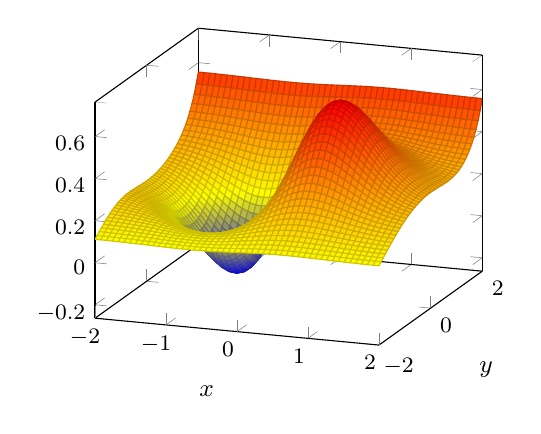
\begin{tikzpicture}
                    \begin{axis}[
                            %title={$x \exp(-x^2-y^2)$},
                            xlabel=$x$, ylabel=$y$,
                            small,
                            view={20}{20}
                        ]
                        \addplot3[surf,domain=-2:2,domain y=-2:2,samples=50]
                        {x*exp(-x*x-y*y) + exp(y*y*y/10)/4} ;
                    \end{axis}
                \end{tikzpicture}
                \caption{$f(x,y) := x e^{-(x^2y^2)}  + \frac{1}{4}e^{y^\frac{3}{10}}$}
            \end{figure}
        \end{column}
    \end{columns}


\end{frame}


\begin{frame}
    \frametitle{Stationary points}


    \begin{columns}
        \begin{column}{.5\textwidth}

            \begin{theorem}
                If \(f:S\to\bR\) is differentiable and has a relative minimum or maximum at \(\aa\), then \(\nabla f(\aa)=  \mathbf{0}\).
            \end{theorem}

            \begin{proof}
                \begin{enumerate}
                    \item Suppose \(f\) has a relative minimum at \(\aa\) (or consider \(-f\));
                    \item For any unit vector \(\vv\) let \(g(u) = f(\aa+u\vv)\);
                    \item \(g\) has relative minimum at \(u=0\) so \(u'(0)=0\);
                    \item This means that \(D_{\vv} f(\aa) = 0\) for every \(\vv\) and so \(\nabla f (\aa)= \mathbf{0}\). \qedhere
                \end{enumerate}
            \end{proof}
        \end{column}
        \begin{column}{.5\textwidth}
            \begin{figure}
                \begin{tikzpicture}
                    \begin{axis}[
                            axis lines=center,
                            small,
                            xlabel=$x$, ylabel=$f(x)$,
                        ]
                        \addplot[
                            blue,
                            domain=-1:1,
                            samples=21,
                        ]
                        {x^3};
                    \end{axis}
                \end{tikzpicture}
                \caption{\(\nabla f(\aa) =  \mathbf{0}\) doesn't imply a minimum or maximum at \(\aa\) as seen for the function \(f(x):=x^3\).}
            \end{figure}
        \end{column}
    \end{columns}

\end{frame}


\begin{frame}
    \frametitle{Stationary points (cont.)}



    \begin{columns}
        \begin{column}{.5\textwidth}

            \begin{definition}[stationary point]
                If \(\nabla f(\aa)=0\) then \(\aa\) is called a \emph{stationary point}.
            \end{definition}



            \begin{figure}
                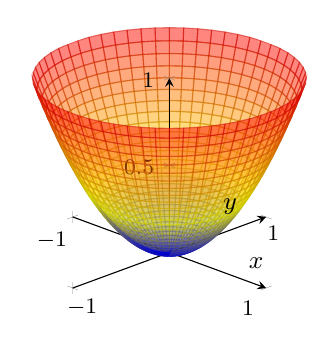
\begin{tikzpicture}
                    \begin{axis}[
                            view={45}{30},
                            axis lines=none,
                            small,
                            xmin=-1, xmax=1,
                            ymin=-1, ymax=1,
                            zmin=0, zmax=1,
                        ]
                        \addplot3[
                            surf,
                            samples=31,                            opacity = 0.5,
                            domain=0:1,y domain=45:225,
                            z buffer=sort,
                        ]
                        ({x * cos(y)},
                        {x * sin(y)},
                        x^2);
                    \end{axis}
                    \begin{axis}[
                            view={45}{30},
                            xlabel=\(x\), ylabel=\(y\),
                            axis lines=center,
                            small,
                            xmin=-1, xmax=1,
                            ymin=-1, ymax=1,
                            zmin=0, zmax=1,
                        ]
                        \addplot3[
                            surf,
                            samples=31,
                            opacity = 0.5,
                            domain=0:1,y domain=225:405,
                            z buffer=auto,
                        ]
                        ({x * cos(y)},
                        {x * sin(y)},
                        x^2);
                    \end{axis}
                \end{tikzpicture}
                \caption{If \(f(x,y)=x^2+y^2\) then \(\nabla f(x,y) = \left(\begin{smallmatrix}
                        2x\\2y
                    \end{smallmatrix}\right)\) and \(\nabla f(0,0) =\left(\begin{smallmatrix}
                        0\\0
                    \end{smallmatrix}\right) \). The point \((0,0)\) is an absolute minimum for \(f\).}
            \end{figure}
        \end{column}
        \begin{column}{.5\textwidth}

            \begin{definition}[saddle point]
                If \(\nabla f(\aa)=0\) and \(\aa\) is neither a minimum nor a maximum then \(\aa\) is said to be a \emph{saddle point}.
            \end{definition}



            \begin{figure}
                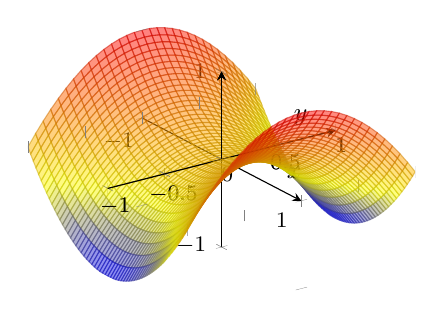
\begin{tikzpicture}
                    \begin{axis}[
                            view={55}{30},
                            axis lines=center,
                            small,
                            xlabel=\(x\), ylabel=\(y\),
                            xmin=-1, xmax=1,
                            ymin=-1, ymax=1,
                            zmin=-1, zmax=1,
                        ]
                        \addplot3[
                            surf,
                            samples=31,
                            opacity = 0.5,
                            domain=-1:0,
                            y domain=-1:1,
                            z buffer=auto,
                        ]
                        {x^2-y^2};
                    \end{axis}
                    \begin{axis}[
                            view={55}{30},
                            axis lines=center,
                            axis x line = none,
                            small,
                            xmin=-1, xmax=1,
                            ymin=-1, ymax=1,
                            zmin=-1, zmax=1,
                        ]
                        \addplot3[
                            surf,
                            samples=31,
                            opacity = 0.5,
                            domain=0:1,
                            y domain=-1:1,
                            z buffer=auto,
                        ]
                        {x^2-y^2};
                    \end{axis}
                \end{tikzpicture}
                \caption{If \(f(x,y)=x^2-y^2\) then \(\nabla f(x,y) = \left(\begin{smallmatrix}
                        2x\\-2y
                    \end{smallmatrix}\right)\) and \(\nabla f(0,0) =\left(\begin{smallmatrix}
                        0\\0
                    \end{smallmatrix}\right) \). The point \((0,0)\) is a saddle point for \(f\).}
            \end{figure}



        \end{column}
    \end{columns}


\end{frame}

\subsection{Second order Taylor formula and Hessian matrix}


\begin{frame}
    \frametitle{Hessian matrix}


    \begin{definition}[Hessian matrix]
        Let \(f:\bR^n \to\bR\) be twice differentiable.
        The \emph{Hessian matrix} at \(\aa\in \bR^n\) is defined
        \[
            \mathbf{H} f (\aa)= \begin{pmatrix}
                \dfrac{\partial^2 f}{\partial x_1^2} (\aa)
                 & \dfrac{\partial^2 f}{\partial x_1\,\partial x_2} (\aa)
                 & \cdots
                 & \dfrac{\partial^2 f}{\partial x_1\,\partial x_n}(\aa)  \\[2.2ex]
                \dfrac{\partial^2 f}{\partial x_2\,\partial x_1} (\aa)
                 & \dfrac{\partial^2 f}{\partial x_2^2}(\aa)
                 & \cdots
                 & \dfrac{\partial^2 f}{\partial x_2\,\partial x_n}(\aa)  \\[2.2ex]
                \vdots
                 & \vdots
                 & \ddots
                 & \vdots                                                 \\[2.2ex]
                \dfrac{\partial^2 f}{\partial x_n\,\partial x_1} (\aa)
                 & \dfrac{\partial^2 f}{\partial x_n\,\partial x_2} (\aa)
                 & \cdots
                 & \dfrac{\partial^2 f}{\partial x_n^2}(\aa)
            \end{pmatrix}.
        \]
    \end{definition}


    \begin{columns}
        \begin{column}{.5\textwidth}
            \begin{itemize}
                \item The Hessian matrix \(\mathbf{H} f (\aa)\) is symmetric;
            \end{itemize}

        \end{column}
        \begin{column}{.5\textwidth}
            \begin{itemize}
                \item If \(\vv= \left( \begin{smallmatrix}
                              v_1\\ \vdots \\v_n
                          \end{smallmatrix} \right)  \) then \(\vv^{\mathbf{t}} \ \mathbf{H} f (\aa) \ \vv \in \bR\).
            \end{itemize}

        \end{column}
    \end{columns}

\end{frame}


\begin{frame}
    \frametitle{\(\vv^{\mathbf{t}} \ \mathbf{H} f (\aa) \ \vv\)}

    %We consider the \(\bR^2\) case. 
    Let \(\vv= \left( \begin{smallmatrix}
            v_1\\ \vdots \\v_n
        \end{smallmatrix} \right)  \).
    We use the notation
    \(\partial_{j}\partial_{k}f(\aa) = \frac{\partial^2 f}{\partial x_j\,\partial x_k} (\aa)\).

    Then
    \[
        \begin{aligned}
            \vv^{\mathbf{t}} \ \mathbf{H} f (\aa) \ \vv
             & =
            \begin{pmatrix}
                v_1 & \cdots & v_n
            \end{pmatrix}
            \begin{pmatrix}
                \partial_{1}\partial_{1}f(\aa) & \cdots &
                \partial_{1}\partial_{n}f(\aa)                   \\
                \vdots                         & \ddots & \vdots \\
                \partial_{n}\partial_{1}f(\aa) & \cdots &
                \partial_{n}\partial_{n}f(\aa)
            \end{pmatrix}
            \begin{pmatrix}
                v_1 \\ \vdots \\v_n
            \end{pmatrix} \\
             & = \sum_{j,k=0}^{n}
            \partial_{j}\partial_{k}f(\aa)
            v_j v_k.
        \end{aligned}
    \]


\end{frame}

\begin{frame}
    \frametitle{Hessian matrix (cont.)}

    \begin{example}
        Let \(f(x,y)=x^2-y^2\).
        The gradient is
        \[\nabla f(x,y) =\begin{pmatrix}
                \frac{\partial f}{\partial x} (x,y) \\[2.2ex]
                \frac{\partial f}{\partial y} (x,y)
            \end{pmatrix} =   \begin{pmatrix}
                2x \\-2y
            \end{pmatrix}.
        \]
        The Hessian is
        \[
            \mathbf{H} f (x,y)= \begin{pmatrix}
                \dfrac{\partial^2 f}{\partial x^2} (x,y)
                 & \dfrac{\partial^2 f}{\partial x\,\partial y} (x,y)
                \\[2.2ex]
                \dfrac{\partial^2 f}{\partial y\,\partial x} (x,y)
                 & \dfrac{\partial^2 f}{\partial y^2}(x,y)
            \end{pmatrix}
            = \begin{pmatrix}
                2
                 & 0
                \\[2.2ex]
                0
                 & -2
            \end{pmatrix}.
        \]
        The point \((0,0)\) is a stationary point since \(\nabla f(0,0) =\left(\begin{smallmatrix}
                0\\0
            \end{smallmatrix}\right) \).
    \end{example}

\end{frame}

\begin{frame}
    \frametitle{Second order Taylor formula for scalar fields}

    \structure{Recall first order Taylor approximation:}
    If \(f\) is differentiable at \(\aa\)
    then
    \(  f(\aa+  \vv) - f(\aa)  = \nabla f(\aa) \cdot \vv + \norm{\vv}E(\aa,\vv)\).
    If \(\aa\) is a stationary point then this only tells us that \(  f(\aa+  \vv) - f(\aa)  =  \norm{\vv}E(\aa,\vv)\) but we want better information.

    \begin{theorem}[second order Taylor]
        Let \(f\) be a scalar field twice differentiable on \(B(\aa,r)\).
        Then, if \(\norm{\vv}\leq r\),
        \[
            f(\aa+\vv) = f(\aa) + \nabla f(\aa) \cdot \vv + \frac{1}{2} \vv^{\mathbf{t}} \ \mathbf{H} f (\aa) \ \vv + \norm{\vv}^2 E_2(\aa,\vv)
        \]
        and \(E_2(\aa,\vv) \to 0\) as \(\norm{\vv}\to 0\).
    \end{theorem}

\end{frame}


\begin{frame}
    \frametitle{}

    \begin{proof}[Proof of second order Taylor formula]

        \begin{enumerate}
            \item Let \(g(u) = f(\aa + u \vv)\);
            \item Taylor's expansion \(g(1) = g(0) + g'(0) + \frac{1}{2} g''(c)\) for some \(c\in (0,1)\);
            \item Since \(g(u) = f(a_1 + uv_1, \ldots, a_n + u v_n)\), by the chain rule,
                  \[
                      g'(u) = \sum_{j=1}^{n} \partial_j f( a_1 + uv_1, \ldots, a_n + u v_n ) v_j
                      =\nabla f( \aa + u \vv) \cdot \vv;
                  \]
                  \vspace{-2em}
            \item Similarly
                  \vspace{-1em}
                  \[
                      g''(u) = \sum_{j,k=1}^{n} \partial_j\partial_k f( a_1 + uv_1, \ldots, a_n + u v_n ) v_j v_k
                      =  \vv^{\mathbf{t}} \ \mathbf{H} f (\aa + u \vv) \ \vv;
                  \]
                  \vspace{-1em}
            \item Consequently
                  \(
                  f(\aa+\vv) = f(\aa) + \nabla f(\aa) \cdot \vv + \frac{1}{2} \vv^{\mathbf{t}} \ \mathbf{H} f (\aa + c\vv) \ \vv
                  \);
            \item We define \(E_2(\aa,\vv) = \frac{1}{2} \frac{1}{\norm{\vv}^2} \vv^{\mathbf{t}} (\mathbf{H} f (\aa + c\vv) - \mathbf{H} f (\aa)  ) \vv\).
            \item \(\abs{E_2(\aa,\vv)} \leq \sum_{j,k=0}^{n}
                  \frac{v_j v_k}{\norm{\vv}^2} \left( \partial_{j}\partial_{k}f(\aa+c\vv)-\partial_{j}\partial_{k}f(\aa) \right).\)
                  \qedhere
        \end{enumerate}
    \end{proof}
\end{frame}

\subsection{Classifying stationary points}


\begin{frame}
    \frametitle{Classifying stationary points}


    \begin{theorem}
        Let \(A\) be a real symmetric matrix and let
        \(Q(\vv) =  \vv^{\mathbf{t}} A  \vv  \).
        Then
        \begin{itemize}
            \item \(Q(\vv) > 0\) for all \(\vv \neq \mathbf{0}\) if and only if all eigenvalues of \(A\) are positive;
            \item \(Q(\vv) < 0\) for all \(\vv \neq \mathbf{0}\) if and only if all eigenvalues of \(A\) are negative.
        \end{itemize}
    \end{theorem}

    \begin{proof}
        \begin{enumerate}
            \item \(A\) can be diagonalised by  matrix \(B\)  which is orthogonal (\(B^{\mathbf{t}}=B^{-1}\))
                  \[
                      D = B^{\mathbf{t}} A B =
                      \begin{pmatrix}
                          \lambda_1 & \cdots & 0         \\
                          \vdots    & \ddots & \vdots    \\
                          0         & \cdots & \lambda_n
                      \end{pmatrix};
                  \]
                  \vspace{-1em}
            \item \(Q(\vv) = \vv^{\mathbf{t}} B^{\mathbf{t}} B A B^{\mathbf{t}} B \vv  = \ww^{\mathbf{t}} D \ww = \sum_{j} \lambda_j w_j^2  \) where \(\ww = B \vv\);
            \item If all \(\lambda_j >0\) then \( \sum_{j} \lambda_j w_j^2  >0\);
            \item \(Q(B \uu_k ) = \lambda_k\) so, if \(Q(\vv) > 0\) for all \(\vv \neq \mathbf{0}\) then \(\lambda_k>0\) for all \(k\). \qedhere
        \end{enumerate}
    \end{proof}

\end{frame}

\begin{frame}
    % \frametitle{Classifying stationary points (cont.)}

    \begin{theorem}[classification of stationary points]
        Let \(f\) be a scalar field twice differentiable on \(B(\aa,r)\).
        Suppose  \(\nabla f(\aa) = \mathbf{0}\).
        Then
        \begin{itemize}
            \item \emph{All} eigenvalues of \(\mathbf{H} f (\aa)\) are positive then \(f\) has a relative minimum at \(\aa\);
            \item \emph{All} eigenvalues of \(\mathbf{H} f (\aa)\) are negative then \(f\) has a relative maximum at \(\aa\);
            \item Some eigenvalues positive and some negative then \(\aa\) is a saddle point.
        \end{itemize}
    \end{theorem}

    \begin{proof}
        \begin{enumerate}
            \item Let \(Q(\vv) =  \vv^{\mathbf{t}} \mathbf{H} f (\aa) \vv  \),  \(\ww = B \vv\) and let \(\Lambda := \min_j \lambda_j\);
            \item Observe that \(\norm{\ww} =  \norm{\vv}\) and that \(Q(\vv)=  \sum_{j} \lambda_j w_j^2  \geq \Lambda \sum_{j} w_j^2 = \Lambda  \norm{\vv}^2 \);
            \item 2\textsuperscript{nd}-order Taylor
                  \vspace{-1em}
                  \[
                      f(\aa+\vv) - f(\aa)
                      =  \frac{1}{2} \vv^{\mathbf{t}} \ \mathbf{H} f (\aa) \ \vv + \norm{\vv}^2 E_2(\aa,\vv)
                      \geq  \left(\tfrac{\Lambda}{2} - E_2(\aa,\vv) \right) \norm{\vv}^2;
                  \]
            \item Since \(E_2(\aa,\vv) \to 0\) as \(\norm{\vv}\to 0\), \(\abs{E_2(\aa,\vv)} < \tfrac{\Lambda}{2}\) when \(\norm{\vv}\) is small.
        \end{enumerate}
        Analogous argument for the second part. For final part consider \(\vv_j\) which is eigenvector for \(\lambda_j\) and apply the argument of first or second part.
    \end{proof}

\end{frame}

\subsection{Extreme value theorem for continuous scalar fields}

\begin{frame}
    \frametitle{Extreme value theorem for continuous scalar fields}

    The argument will be in two parts:
    \begin{enumerate}
        \item Continuity implies boundedness;
        \item Boundedness implies that the maximum and minimum are attained.
    \end{enumerate}

    \structure{Notation:}
    Intervals / rectangles / etc\ldots
    If \(\aa = (a_1,\ldots,a_n)\) and  \(\bb = (b_1,\ldots,b_n)\)
    then we consider the \(n\)-dimensional closed cartesian product
    \[
        [\aa,\bb] = [a_1,b_1] \times \cdots \times [a_n,b_n].
    \]
    We call this set a \emph{rectangle}.

\end{frame}

\begin{frame}
    \frametitle{}

    \begin{theorem}[Bolzano–Weierstrass]
        If \({\{\xx_{n}\}}_{n}\) is a sequence in \( [\aa,\bb]\)
        there exists a convergent subsequence \({\{\xx_{n_j}\}}_{j}\).
    \end{theorem}

    \begin{columns}

        \begin{column}{.5\textwidth}
            \begin{proof}
                \begin{enumerate}
                    \item Divide \( [\aa,\bb]\) into sub-rectangles of size half the original;
                    \item Choose a sub-rectangle which contains infinite elements of the sequence and choose the first of these elements to be part of the sub-sequence;
                    \item Now divide again this sub-rectangle by half and repeat to give the subsequence.
                \end{enumerate}
            \end{proof}
        \end{column}

        \begin{column}{.5\textwidth}
            [Insert: illustration of proof]
        \end{column}
    \end{columns}

\end{frame}

\begin{frame}
    \frametitle{Boundedness}

    \begin{theorem}[boundedness of continuous scalar fields]
        Suppose that \(f\) is a scalar field continuous at every point in the closed rectangle \([\aa,\bb]\).
        Then \(f\) is bounded on \([\aa,\bb]\) in the sense that there exists \(C>0\) such that \(\abs{f(\xx)} \leq C\) for all \(\xx \in [\aa,\bb]\).
    \end{theorem}


    \begin{proof}
        \begin{enumerate}
            \item Suppose the contrary: for all \(n\in\bN\) there exists \(\xx_n\in [\aa,\bb]\) such that \(\abs{f(\xx_n)}>n\);
            \item Bolzano–Weierstrass theorem means that there exists a subsequence \({\{\xx_{n_j}\}}_{j}\) converges to \( \xx \in [\aa,\bb]\);
            \item Continuity of \(f\) means that \(f(\xx_{n_j})\) converges to \(f(\xx)\). This is a contradiction.
        \end{enumerate}



    \end{proof}

\end{frame}

\begin{frame}
    \frametitle{Attaining extreme values}

    \begin{theorem}[extreme value theorem]
        Suppose that \(f\) is a scalar field continuous at every point in the closed rectangle \([\aa,\bb]\).
        There there exist points \( \xx, \yy \in [\aa,\bb]\) such that
        \[
            f(\xx) = \inf f
            \quad \text{and} \quad
            f(\yy)= \sup f.
        \]
    \end{theorem}

    \begin{proof}
        \begin{itemize}
            \item  By the boundedness theorem \(\sup f\) is finite and so there exists a sequence  \({\{\xx_{n}\}}_{n}\)  such that \(f(\xx_n)\) converges to \(\sup f\);
            \item Bolzano–Weierstrass theorem implies that there exists a subsequence  \({\{\xx_{n_j}\}}_{j}\) which converges to \( \xx \in [\aa,\bb]\);
            \item By continuity \(f(\xx_n) \to f(\xx) = \sup f\).
        \end{itemize}
    \end{proof}


\end{frame}

\section{Extrema with constraints}

\subsection{Lagrange multipliers}


\begin{frame}
    \frametitle{The geometric idea of Lagrange multipliers}

    \begin{columns}
        \begin{column}{.5\textwidth}
            \begin{figure}
                \noindent\begin{tikzpicture}%
                    \node[anchor=south west,inner sep=0] (image) at (0,0)
                    {\includesvg[width=\textwidth,inkscapelatex=false]{lagrange}};
                    % SVG adapted from work in public domain (https://commons.wikimedia.org/wiki/File:LagrangeMultipliers2D.svg)
                    \begin{scope}[x={(image.south east)},y={(image.north west)}]
                        % scope for unitary coordinates over image
                        \node[] at (0.37,.52) {\(\nabla f\)};
                        \node[] at (0.57,.48) {\color{red}\(\nabla g\)};
                        \node[] at (0.44,0.74) {\(f=c_3\)};
                        \node[] at (0.85,0.9) {\color{red}\( g(x,y)=0\)};
                        \node[] at (0.4,0.9) {\(f=c_2\)};
                        \node[] at (0.15,0.98) {\(f = c_1\)};
                    \end{scope}
                \end{tikzpicture}
                \caption{Extrema of \(f\) under constraint \(g\)}
            \end{figure}

        \end{column}
        \begin{column}{.5\textwidth}
            \structure{Problem:}
            Minimise (or maximise) \(f(x,y)\) under the constraint \(g(x,y) = 0\).
            \begin{itemize}
                \item At ``touching point'' the gradient vectors are parallel;
                \item I.e., \(\nabla f = \lambda \nabla g\) for some \(\lambda \in \bR\).
            \end{itemize}
        \end{column}
    \end{columns}


\end{frame}



\begin{frame}
    \frametitle{Lagrange multipliers}


    \begin{block}{Method of Lagrange's multipliers}
        If a scalar field \(f(x_1,\ldots,x_n)\) has a relative extremum when it is subject to \(m\) constraints
        \[
            g_1(x_1,\ldots,x_n) = 0,
            \dots , g_m(x_1,\ldots,x_n)=0,
        \]
        where \(m<n\), then there exist \(m\) scalars \(\lambda_1,\ldots,\lambda_m\) such that
        \[
            \nabla f = \lambda_1 \nabla g_1 + \cdots + \lambda_m \nabla g_m
        \]
        at the extremum point.
    \end{block}



\end{frame}



\begin{frame}
    \frametitle{Lagrange multipliers (cont.)}

    \begin{example}
        Find the extrema of \(f(x,y) = xy\) subject to the constraint \(g(x,y) = x+y-1 =0\).
        \begin{itemize}
            \item \(\nabla f(x,y) = \left(\begin{smallmatrix}
                      y\\ x
                  \end{smallmatrix}\right)\)
                  and \(\nabla g(x,y) = \left(\begin{smallmatrix}
                      1\\ 1
                  \end{smallmatrix}\right)\);
            \item  According to the Lagrange multiplier method there is \(\lambda\in \bR\) such that \(\nabla f(x,y) = \lambda \nabla g(x,y)\) at the extremum point \((x,y)\);
            \item We must solve the simultaneous equations
                  \[
                      \left(\begin{smallmatrix}
                              y\\ x
                          \end{smallmatrix}\right)
                      = \lambda \left(\begin{smallmatrix}
                              1\\ 1
                          \end{smallmatrix}\right),
                      \quad g(x,y) =0;
                  \]
            \item I.e.,
                  \( x = \lambda, \quad
                  y = \lambda, \quad
                  x+y = 1;
                  \)
            \item This has the solution \((x,y) = (\frac{1}{2},\frac{1}{2})\), \(f(\frac{1}{2},\frac{1}{2})= \frac{1}{4}\).
        \end{itemize}
    \end{example}

\end{frame}

\begin{frame}
    \frametitle{Lagrange multipliers (cont.)}

    \begin{example}
        Find the points closest and furthest from the origin on the curve defined by the intersection of the two surfaces
        \[
            x^2 - xy + y^2 - z^2 = 1
            \quad \text{and} \quad
            x^2 + y^2 = 1.
        \]
        \vspace{-1em}
        \begin{itemize}
            \item Let \(f(x,y,z) = \sqrt{x^2 + y^2 + z^2}\);
            \item Let \(g_1(x,y,z) = x^2 - xy + y^2 - z^2 - 1\),
                  \(g_2(x,y,z) = x^2 + y^2 - 1\);
            \item Calculate \(\nabla f\), \(\nabla g_1\) and \(\nabla g_2\);
            \item Solve the system of 5 equations (and 5 unknowns):
                  \vspace{-1em}
                  \[
                      \nabla f (x,y,z) = \lambda_1 \nabla g_1(x,y,z)  + \lambda_2 \nabla g_2(x,y,z),
                  \]
                  \[
                      \quad g_1(x,y,z) =0,
                      \quad g_2(x,y,z) =0;
                  \]
            \item Check which are closest to and which are furthest from the origin.
        \end{itemize}
    \end{example}


\end{frame}

\end{document}
